\documentclass[xcolor=table, hyperref={pdfpagelabels=false}]{beamer}
\usepackage{lmodern}
\usepackage{amssymb}
\usepackage[style=alphabetic,
citestyle=authoryear]{biblatex}
\renewcommand*{\bibfont}{\scriptsize}
\addbibresource{bibliography.bib}

\usepackage{tikz}
\usetikzlibrary{decorations.pathreplacing}
\usetikzlibrary{shapes,arrows}
\definecolor{myLightGray}{RGB}{191,191,191}
\definecolor{myGray}{RGB}{160,160,160}
\definecolor{myDarkGray}{RGB}{144,144,144}
\definecolor{myDarkRed}{RGB}{167,114,115}
\definecolor{myRed}{RGB}{255,58,70}
\definecolor{myGreen}{RGB}{0,255,71}
\usepackage{lmodern}
\usepackage{amsmath}
\usepackage{dsfont}
\usepackage{marvosym}
\usepackage{subcaption}
\usepackage{ stmaryrd }

\usepackage[utf8]{inputenc}
\usetheme{Frankfurt}
\usepackage{qtree}
\usepackage{subcaption}
\newcommand\SmallCaption[1]{%
	\captionsetup{font=scriptsize}%
	\caption{#1}}



\title{Semantics and pragmatics of numerical approximation expressions}  
\author[a]{Adèle Mortier\\[10mm]{\small Supervisors:\\ Paul Égré $|$ Benjamin Spector}}



\date{\today} 
\begin{document}

\begin{frame}
\titlepage

\end{frame} 






\begin{frame}{A first example}
\begin{center}
	\huge ``I got it for around 10 \EUR''
\end{center}\pause
\begin{block}{What you think of this}
	\begin{itemize}
		\item She does not know for sure how much it cost\pause
		\item It does not matter so much\pause
		\item \textbf{She is too ``lazy'' to say the exact amount and is counting on me to understand correctly}
	\end{itemize}
\end{block}\pause
\begin{block}{What you understand}
	Between 8 and 12 \EUR?\\
	$\triangleright$ We would like to derive this in a systematic way !
\end{block}
\end{frame}
\begin{frame}
\frametitle{Table of contents}
\tableofcontents
\end{frame} 
\section{Setting the problem} 
\begin{frame}{}
\begin{center}
	\Huge Setting the problem
\end{center}
\end{frame}
\begin{frame}{Parameters et hypotheses}\vspace{-3mm}
\begin{center}
	Around (10) (people) (came to the party)
\end{center}\vspace{-4mm}
\begin{eqnarray*}
	\llbracket \mbox{around } n \mbox{ Ps did Q}\rrbracket^{\epsilon} &=& 1 \mbox{ iff } |P \cap Q| \in [n-\epsilon(n); n+\epsilon(n)]\\
	&\triangleq& 1 \mbox{ iff } |P \cap Q| \in \mathcal{A}^n_{\epsilon}
\end{eqnarray*}\vspace{-8mm}
\begin{block}{Basic semantics}
	\begin{itemize}
		\item Denotes an interval centered on n, size 2$\epsilon$(n)+1
		\item $\epsilon$ depends on n !!
	\end{itemize}
\end{block}\pause
\begin{exampleblock}{Dependencies}
	\begin{itemize}
		\item \textbf{Order of magnitude}: the bigger the n, the wider  the interval\pause
		\item \textbf{Granularity}: the coarser the n, the wider the interval\pause
		\item \textbf{Salience}: in presence of a salient alternative, narrower interval (\cite{cummins2012})
	\end{itemize}
\end{exampleblock}
\end{frame}
\begin{frame}{Toy dataset}
\begin{center}
\begin{tabular}{lllcl}
	(Magnitude) & I got it for &600,000 \EUR &\textit{vs}& 10\EUR \pause \\ 
(Granularity) & I got it for &600,000 \EUR &\textit{vs}& 600,050 \EUR \pause \\ 
(Salience) & \multicolumn{3}{l}{$[$Ideal budget: 560,000 \EUR$]$}& got it for 600,000 \EUR \pause
\end{tabular}
\end{center}
\begin{block}{Consequences}
	\begin{itemize}
		\item Granularity and magnitude are intertwined (which one is predominant??)
		\item Granularity and salience are implicature-based
	\end{itemize}
\end{block}\vspace{-3mm}
\begin{figure}[H]
	\centering
	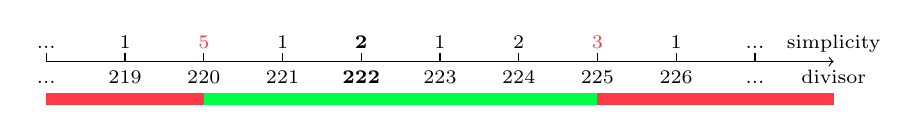
\begin{tikzpicture}[%
	every node/.style={
		font=\scriptsize,
		% Better alignment, see https://tex.stackexchange.com/questions/315075
		text height=1ex,
		text depth=.25ex,
	},
	]
	% draw horizontal line   
	\draw[->] (0,0) -- (10,0);
	
	% draw vertical lines
	\foreach \x in {0,1,...,9}{
		\draw (\x cm,3pt) -- (\x cm,0pt);
	}
	
	% place axis labels
	\node[anchor=north] at (0,0) {...};
	\node[anchor=south] at (0,0) {...};
	
	\node[anchor=north] at (1,0) {219};
	\node[anchor=south] at (1,0) {1};
	
	\node[anchor=north] at (2,0) {220};
	\node[anchor=south] at (2,0) {\textcolor{myRed}{5}};
	
	\node[anchor=north] at (3,0) {221};
	\node[anchor=south] at (3,0) {1};
	
	\node[anchor=north] at (4,0) {\textbf{222}};
	\node[anchor=south] at (4,0) {\textbf{2}};
	
	\node[anchor=north] at (5,0) {223};
	\node[anchor=south] at (5,0) {1};
	
	\node[anchor=north] at (6,0) {224};
	\node[anchor=south] at (6,0) {2};
	
	\node[anchor=north] at (7,0) {225};
	\node[anchor=south] at (7,0) {\textcolor{myRed}{3}};
	
	\node[anchor=north] at (8,0) {226};
	\node[anchor=south] at (8,0) {1};
	
	\node[anchor=north] at (9,0) {...};
	\node[anchor=south] at (9,0) {...};
	
	\node[anchor=north] at (10,0) {divisor};
	\node[anchor=south] at (10,0) {simplicity};
	% draw scale below
	\fill[myGreen] (2,-0.4) rectangle (7,-0.55);
	\fill[myRed] (0,-0.4) rectangle (2,-0.55);
	\fill[myRed] (7,-0.4) rectangle (10,-0.55);
	\end{tikzpicture}
	\caption{Interval inferred for ``around 222'' using granularity implicatures}
\end{figure}
\end{frame}
\section{Two Bayesian models}
\begin{frame}
\begin{center}{}
	\Huge Two Bayesian models
\end{center}
\end{frame}
\begin{frame}{Probabilistic intervals (\cite{egre2018})}
\begin{block}{Principle: 2 levels}
	\begin{itemize}
		\item When the speaker utters ``around n'', he thinks of a certain interval among a \textbf{set of possible intervals} (\textit{e.g.} intervals centered around n); \pause
		\item According to the listener, \textbf{each possible interval has a certain probability} (\textit{e.g.} relatively narrow intervals might be more probable); \pause
		\item And within a fixed interval, the \textbf{``real'' number} is selected with a certain probability (\textit{e.g.} central numbers might be more probable)
	\end{itemize}
\end{block}
	\begin{figure}
	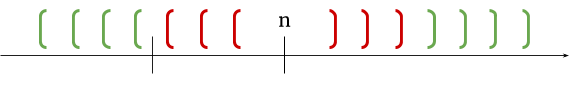
\includegraphics[width=\textwidth]{./images/intervals.png}
\end{figure}
\end{frame}
\begin{frame}{Properties of the model}\vspace{-3mm}
	\begin{figure}
		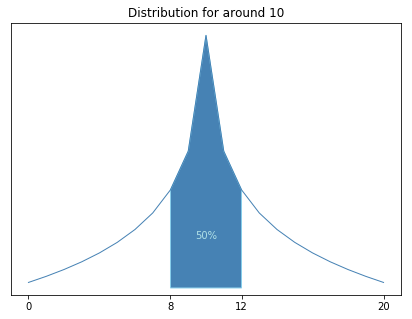
\includegraphics[width=.45\textwidth]{./images/around_10_prob_simple.png}
		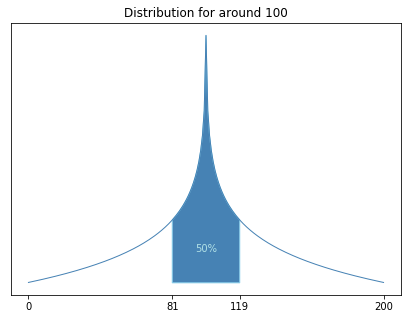
\includegraphics[width=.45\textwidth]{./images/around_100_prob_simple.png}
		\caption{Curves generated using uniform distributions on intervals and numbers}
	\end{figure}
\vspace{-8mm}
	\begin{block}{Properties}
		\begin{itemize}
			\item Symmetrical \pause
			\item Scales with magnitude \pause
			\item Does not account for granularity
		\end{itemize}
	\end{block}
\end{frame}
\begin{frame}{Refinements}
\begin{block}{Behind Bayes}
	\begin{equation*}
		\mathds{P}[k] = \sum_{i = |n-k|}^n \mathds{P}[k|\mathcal{A}^n_i]\mathds{P}[\mathcal{A}^n_i]
		= -\alpha \ln(-2k + \beta) + \gamma \footnote{\begin{small}
			$\alpha = \frac{1}{2(n+1)}$
			$\beta = 2n+1$
			$\gamma = \frac{\ln (2n+1)}{2(n+1)} = \alpha \ln(\beta)$
			\end{small}}
	\end{equation*}
		Hints at the Weber-Fechner law and numerical cognition?? (\cite{dehaene2003})
\end{block}\pause
\begin{exampleblock}{Related models}
	\begin{itemize}
		\item change distributions\pause
		\item relax the constraints on possible intervals\pause
		\item higher-order uncertainty on the set of intervals
	\end{itemize}
\end{exampleblock}
\end{frame}
\begin{frame}{The Rational Speech Acts (RSA) model}
\begin{block}{Principle (\cite{lassiter2013,bergen2016})}\pause
	\begin{itemize}
		\item one set of \textbf{utterances} (each with a cost and possible meanings), one set of \textbf{observations} (numbers), one set of \textbf{thresholds} (numbers); \pause
		\item mutually recursive Bayesian updates \pause
		\item optimality = tradeoff between \textbf{cost} and \textbf{informativity}
	\end{itemize}
\end{block}
\begin{figure}
	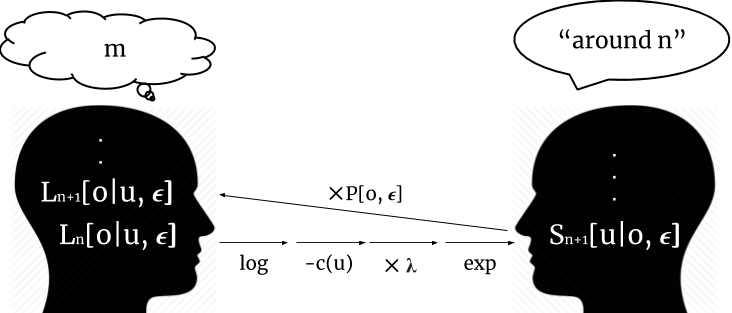
\includegraphics[width=.8\textwidth]{./images/rsa.png}
\end{figure}
\end{frame}

\begin{frame}{Results}
\begin{figure}
	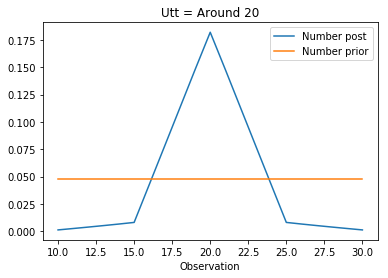
\includegraphics[width=.45\textwidth]{./images/bilateral_around_20_number.png}
	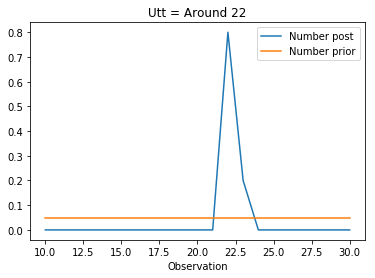
\includegraphics[width=.45\textwidth]{./images/bilateral_around_22_number.png}
\end{figure}\pause
\begin{block}{Properties}
	\begin{itemize}
		\item Accounts for GR (hardcoded in the cost!)\pause
		\item (Almost) symmetrical
	\end{itemize}
\end{block}
\end{frame}
\section{Main goals}
\begin{frame}{}
\begin{center}
	\Huge Main goals
\end{center}
\end{frame}

\begin{frame}{Under quantification}
\begin{center}
	\#The child ate around 17 candies \\ \vspace{2mm}
	All children ate around 17 candies \\
	All children ate around 20 candies \\ \vspace{2mm}
	All children ate between 16 and 18 candies \\
	All children ate between 16 and 24 candies \\
\end{center}
\begin{alertblock}{Strange behavior}
	\begin{itemize}
		\item with around, no ``granularity violation'': a number with minimum granularity can be approximated !\pause
		\item with around, \textbf{opinionatedness} of the speaker about each number, with between, \textbf{ignorance inference};\pause
		\item not a mere disjunction of numbers: it seems possible that no child ate exactly 17 candies !\pause
		\item fine-grained, introspective data (what do people think of it?)
	\end{itemize}
\end{alertblock}
\end{frame}
\begin{frame}{Conclusion}
\begin{block}{Conclusion}
	\begin{itemize}
		\item probabilistic models work for \textbf{basic inferences} on numbers;\pause
		\item but we need some additional refinements to account for \textbf{epistemic inferences}...\pause
		\item ... and for the difference between ``around'' and ``between''!\pause
		\item a small (controlled, pre-registered) experiment might be envisaged to obtain clearer judgements about these contrasts.
	\end{itemize}
\end{block}
\end{frame}
\begin{frame}[allowframebreaks]
\frametitle{Selected references}
\nocite{*}

\printbibliography
\end{frame}

\section{Appendices}
\begin{frame}{Probabilistic unconstrained intervals}
\begin{figure}
	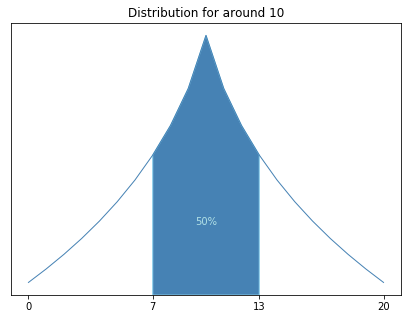
\includegraphics[width=.45\textwidth]{./images/around_10_prob_unconstrained.png}
	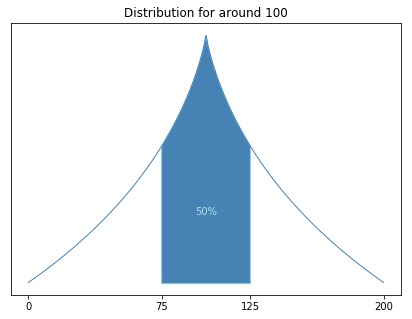
\includegraphics[width=.45\textwidth]{./images/around_100_prob_unconstrained.png}
\end{figure}

\begin{block}{Properties}
	\begin{itemize}
		\item intervals containing n, but not necessarily centered around n;
		\item scales with magnitude;
		\item less peaked.
	\end{itemize}
\end{block}
\end{frame}
\begin{frame}{RSA formulae}
\begin{equation*}
\begin{array}{rcl}
L_0[o|u, \epsilon] &\propto& \mathds{1}_{\lbrace o \in [\llbracket u \rrbracket - \epsilon; \llbracket u \rrbracket + \epsilon]\rbrace} . \mathds{P}[o] \\
\forall n \in \mathds{N}^+, \ S_n[u|o, \epsilon] &\propto& \exp \left( \lambda (\log(L_{n-1}[o|u,\epsilon]) - c(u))\right)\\
\forall n \in \mathds{N}^+, \ L_n[o|u, \epsilon] &\propto& S_n[u|o, \epsilon ] .\mathds{P}[o, \epsilon]
\end{array}
\end{equation*}
\begin{block}{Explanations}
	\begin{itemize}
		\item first step: for fixed u (e.g. ``around x'') and $\epsilon$, just keep the observations that are in [n-$\epsilon$; n+$\epsilon$]; all the other have 0 probability.
		\item speaker step: the softmax allows to pick some non optimal possibilities with a non-zero (but very small) probability
	\end{itemize}
\end{block}
\end{frame}
\begin{frame}{RSA with quantifiers (replication)}
\begin{minipage}{.5\textwidth}
	\begin{figure}
	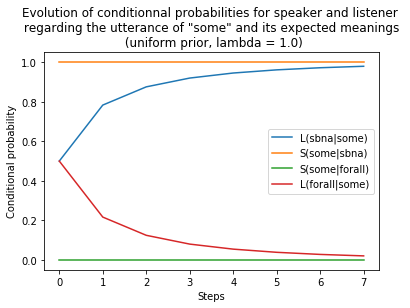
\includegraphics[width=\textwidth]{./images/quantification_lambda_1.png}
\end{figure}
\end{minipage}
\begin{minipage}{.48\textwidth}
	\begin{block}{Some \textit{vs} all}
	\begin{itemize}
		\item at the beginning, ``some'' can mean all ($\forall$) are some but not all ($\exists_{\neg \forall}$), and ``all'' definitely means $\forall$.
		\item this asymmetry causes the meaning of ``some'' to converge to $\exists_{\neg \forall}$ after a few iterations.
	\end{itemize}
\end{block}
\end{minipage}
\begin{alertblock}{\textit{Caveats}}
	\begin{itemize}
		\item Sensitive to parameter $\lambda$!
		\item $\lambda$ is the temperature, higher $\lambda$ means faster convergence but possibly to a ``wrong'' optimum.
	\end{itemize}
\end{alertblock}
\end{frame}
\begin{frame}{RSA with gradable adjectives (replication)}\vspace{-3mm}
\begin{figure}
		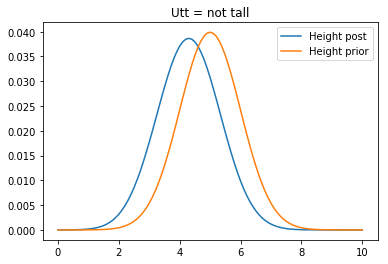
\includegraphics[width=.45\textwidth]{./images/unilateral_not_tall_height.png}
		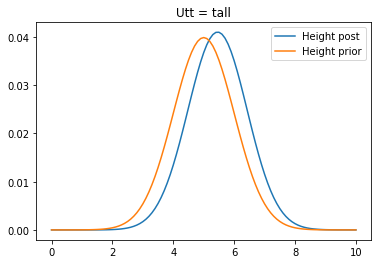
\includegraphics[width=.45\textwidth]{./images/unilateral_tall_height.png}
\end{figure}\vspace{-6mm}
\begin{block}{Properties}
	\begin{itemize}
		\item A negative utterance (``not tall''), shifts the height prior to the \textbf{left}: the listener expects the person to be \textbf{smaller};
		\item A positive utterance (``tall''), shifts the height prior to the \textbf{right}: the listener expects the person to be \textbf{taller};
		\item ``Not tall'' has a bigger effect on the prior, because it is more costly. If it has been uttered, then the person is \textit{really} small
	\end{itemize}
\end{block}
\end{frame}
\begin{frame}{Quantification}
\begin{table}
	\begin{tabular}{lcl}
	\begin{tabular}{c}
		All children ate\\around n candies
	\end{tabular}
	 &$\sim$& $\left \lbrace \begin{tabular}{l}
	Child $\#$ 1 ate around n$_1$ candies\\
	Child $\#$ 2 ate around n$_2$ candies\\
	\vdots\\
	Child $\#$ M ate around n$_M$ candies
\end{tabular} \right.$
\end{tabular}
\end{table}
Maybe I am saying ``around n'' because:
\begin{equation*}
n \in \cap_{i = 1}^{M} [[ around \ n_i ]]
\end{equation*}
\end{frame}
\begin{frame}{Modality}
\begin{tabular}{lcl}
	You \textbf{can} eat around 20 candies &=& $\exists$ W, [16; 24]\\ &$\leadsto$& $\forall$ W, [0; 24] \vspace{2mm} \\ 
	You \textbf{must} eat around 20 candies &=& $\forall$ W, [16; 24]\\
	&$\leadsto$& $\exists$ W, [24; $\infty$[
\end{tabular}
\begin{alertblock}{Strange behavior}
	\begin{itemize}
		\item under existential modality, approximators rather convey an \textbf{upper bound}
		\item under universal modality, approximators rather convey a \textbf{lower bound}
		\item radically different if we use ``between 16 and 24'' instead !!
	\end{itemize}
\end{alertblock}
\end{frame}
\begin{frame}{Additional data (\cite{solt2017})}
\begin{center}
	Lisa has about 50 sheep.\\
	\# Lisa doesn’t have about 50 sheep.\\
	\# Lisa has more than about 50 sheep.\\
	Lisa doesn't have more than about 50 sheep.
\end{center}
\end{frame}
\end{document}
